\documentclass[]{book}
\usepackage{lmodern}
\usepackage{amssymb,amsmath}
\usepackage{ifxetex,ifluatex}
\usepackage{fixltx2e} % provides \textsubscript
\ifnum 0\ifxetex 1\fi\ifluatex 1\fi=0 % if pdftex
  \usepackage[T1]{fontenc}
  \usepackage[utf8]{inputenc}
\else % if luatex or xelatex
  \ifxetex
    \usepackage{mathspec}
  \else
    \usepackage{fontspec}
  \fi
  \defaultfontfeatures{Ligatures=TeX,Scale=MatchLowercase}
\fi
% use upquote if available, for straight quotes in verbatim environments
\IfFileExists{upquote.sty}{\usepackage{upquote}}{}
% use microtype if available
\IfFileExists{microtype.sty}{%
\usepackage{microtype}
\UseMicrotypeSet[protrusion]{basicmath} % disable protrusion for tt fonts
}{}
\usepackage[unicode=true]{hyperref}
\hypersetup{
            pdftitle={Tutorial from mixed models YouTube series},
            pdfauthor={Jeanette Mumford},
            pdfborder={0 0 0},
            breaklinks=true}
\urlstyle{same}  % don't use monospace font for urls
\usepackage{color}
\usepackage{fancyvrb}
\newcommand{\VerbBar}{|}
\newcommand{\VERB}{\Verb[commandchars=\\\{\}]}
\DefineVerbatimEnvironment{Highlighting}{Verbatim}{commandchars=\\\{\}}
% Add ',fontsize=\small' for more characters per line
\usepackage{framed}
\definecolor{shadecolor}{RGB}{248,248,248}
\newenvironment{Shaded}{\begin{snugshade}}{\end{snugshade}}
\newcommand{\KeywordTok}[1]{\textcolor[rgb]{0.13,0.29,0.53}{\textbf{{#1}}}}
\newcommand{\DataTypeTok}[1]{\textcolor[rgb]{0.13,0.29,0.53}{{#1}}}
\newcommand{\DecValTok}[1]{\textcolor[rgb]{0.00,0.00,0.81}{{#1}}}
\newcommand{\BaseNTok}[1]{\textcolor[rgb]{0.00,0.00,0.81}{{#1}}}
\newcommand{\FloatTok}[1]{\textcolor[rgb]{0.00,0.00,0.81}{{#1}}}
\newcommand{\ConstantTok}[1]{\textcolor[rgb]{0.00,0.00,0.00}{{#1}}}
\newcommand{\CharTok}[1]{\textcolor[rgb]{0.31,0.60,0.02}{{#1}}}
\newcommand{\SpecialCharTok}[1]{\textcolor[rgb]{0.00,0.00,0.00}{{#1}}}
\newcommand{\StringTok}[1]{\textcolor[rgb]{0.31,0.60,0.02}{{#1}}}
\newcommand{\VerbatimStringTok}[1]{\textcolor[rgb]{0.31,0.60,0.02}{{#1}}}
\newcommand{\SpecialStringTok}[1]{\textcolor[rgb]{0.31,0.60,0.02}{{#1}}}
\newcommand{\ImportTok}[1]{{#1}}
\newcommand{\CommentTok}[1]{\textcolor[rgb]{0.56,0.35,0.01}{\textit{{#1}}}}
\newcommand{\DocumentationTok}[1]{\textcolor[rgb]{0.56,0.35,0.01}{\textbf{\textit{{#1}}}}}
\newcommand{\AnnotationTok}[1]{\textcolor[rgb]{0.56,0.35,0.01}{\textbf{\textit{{#1}}}}}
\newcommand{\CommentVarTok}[1]{\textcolor[rgb]{0.56,0.35,0.01}{\textbf{\textit{{#1}}}}}
\newcommand{\OtherTok}[1]{\textcolor[rgb]{0.56,0.35,0.01}{{#1}}}
\newcommand{\FunctionTok}[1]{\textcolor[rgb]{0.00,0.00,0.00}{{#1}}}
\newcommand{\VariableTok}[1]{\textcolor[rgb]{0.00,0.00,0.00}{{#1}}}
\newcommand{\ControlFlowTok}[1]{\textcolor[rgb]{0.13,0.29,0.53}{\textbf{{#1}}}}
\newcommand{\OperatorTok}[1]{\textcolor[rgb]{0.81,0.36,0.00}{\textbf{{#1}}}}
\newcommand{\BuiltInTok}[1]{{#1}}
\newcommand{\ExtensionTok}[1]{{#1}}
\newcommand{\PreprocessorTok}[1]{\textcolor[rgb]{0.56,0.35,0.01}{\textit{{#1}}}}
\newcommand{\AttributeTok}[1]{\textcolor[rgb]{0.77,0.63,0.00}{{#1}}}
\newcommand{\RegionMarkerTok}[1]{{#1}}
\newcommand{\InformationTok}[1]{\textcolor[rgb]{0.56,0.35,0.01}{\textbf{\textit{{#1}}}}}
\newcommand{\WarningTok}[1]{\textcolor[rgb]{0.56,0.35,0.01}{\textbf{\textit{{#1}}}}}
\newcommand{\AlertTok}[1]{\textcolor[rgb]{0.94,0.16,0.16}{{#1}}}
\newcommand{\ErrorTok}[1]{\textcolor[rgb]{0.64,0.00,0.00}{\textbf{{#1}}}}
\newcommand{\NormalTok}[1]{{#1}}
\usepackage{longtable,booktabs}
\usepackage{graphicx,grffile}
\makeatletter
\def\maxwidth{\ifdim\Gin@nat@width>\linewidth\linewidth\else\Gin@nat@width\fi}
\def\maxheight{\ifdim\Gin@nat@height>\textheight\textheight\else\Gin@nat@height\fi}
\makeatother
% Scale images if necessary, so that they will not overflow the page
% margins by default, and it is still possible to overwrite the defaults
% using explicit options in \includegraphics[width, height, ...]{}
\setkeys{Gin}{width=\maxwidth,height=\maxheight,keepaspectratio}
\IfFileExists{parskip.sty}{%
\usepackage{parskip}
}{% else
\setlength{\parindent}{0pt}
\setlength{\parskip}{6pt plus 2pt minus 1pt}
}
\setlength{\emergencystretch}{3em}  % prevent overfull lines
\providecommand{\tightlist}{%
  \setlength{\itemsep}{0pt}\setlength{\parskip}{0pt}}
\setcounter{secnumdepth}{5}
% Redefines (sub)paragraphs to behave more like sections
\ifx\paragraph\undefined\else
\let\oldparagraph\paragraph
\renewcommand{\paragraph}[1]{\oldparagraph{#1}\mbox{}}
\fi
\ifx\subparagraph\undefined\else
\let\oldsubparagraph\subparagraph
\renewcommand{\subparagraph}[1]{\oldsubparagraph{#1}\mbox{}}
\fi

\title{Tutorial from mixed models YouTube series}
\author{Jeanette Mumford}
\date{2020-01-29}

\begin{document}
\maketitle

{
\setcounter{tocdepth}{1}
\tableofcontents
}
\chapter{Introduction}\label{introduction}

Some words about the tutorials

\chapter{Video 3: Relating two-stage random effects to simulated data
and model
output}\label{video-3-relating-two-stage-random-effects-to-simulated-data-and-model-output}

\section{Introduction}\label{introduction-1}

The purpose of this document is to help in understanding the two-stage
random effects formulation for mixed models by simulating data based on
the formulation, analyzing the simulated data and comparing the two.
This is a great way to wrap your head around what a mixed model is
doing. This is written under the assumption that you have seen the first
few videos in the Mixed Models series on the MumfordBrainStats YouTube
channel. If you haven't, go look for that playlist and watch those
first. As discussed in the videos, this is not a perfect setup for the
mixed models and not all mixed models can fit into this formulation, but
it is a great way to understand mixed models. Sometimes it is helpful to
see how repeated measures data are simulated in order to understand what
the model is doing. In this case the values in the simulation will show
up again when the data are fit using the lmer() function. Make sure to
spend time matching up the values in the simulation code with the lmer
output to increase your understanding of mixed models.

\section{Data simulation}\label{data-simulation}

The simulation follows the two-stage random effects formulation in
reverse to make up some fake data that look similar to the Sleepstudy
data. Typically simulations are used for estimating type I error and
power, but they are great for learning too. The benefit in simulation is
the truth is known and be compared with the estimates. Specifically,the
true group intercept and slope as well as all of the variance parameters
will be known in this case.

\subsubsection{Review of the two-stage
formulation}\label{review-of-the-two-stage-formulation}

Reviewing the two-stage formulation, recall the first stage of the model
is
\(Y_i = Z_i\beta_i + \epsilon_i, \epsilon_i\sim N(0, \sigma^2I_{n_i})\).
In this case \(Y_i\) contains the average reaction times for subject
\(i\) over 10 days, \(Z_i\) is the design matrix with a column of 1s and
a column for days (0-9), \(\beta_i\) is the vector with the slope and
intercept for subject \(i\) and \(\sigma\) is the within-subject
variance. Notably, this variance is assumed to be the same for all
subjects, as it does not have an \(i\) subscript. Last, \(n_i\), the
number of observations for subject \(i\), is assumed to be 10 for all
subjects, so \(I_{n_i}\) is a \(n_i\times n_i\) identity matrix. Here's
an example using the first subject in the data set (\(i\) would be 1),
\[\left[\begin{array}{c}265 \\ 252 \\ 451 \\ 335 \\ 376 \\370 \\ 357 \\ 514 \\ 350 \\ 500 \end{array}\right] = \left[\begin{array}{cc}
1 & 0 \\
1 & 1 \\
1 & 2 \\
1 & 3 \\
1 & 4 \\
1 & 5 \\
1 & 6 \\
1& 7 \\
1 & 8 \\
1 & 9 \end{array}\right]\left[\begin{array}{c}\beta_{0, i} \\ \beta_{1, i}  \end{array}\right] + 
\left[\begin{array}{c}
\epsilon_1 \\
\epsilon_2 \\
\epsilon_3 \\
\epsilon_4 \\
\epsilon_5 \\
\epsilon_6 \\
\epsilon_7 \\
\epsilon_8 \\
\epsilon_9 \\
\epsilon_{10} 
\end{array}\right].\]

The second level is \(\beta_i = A_i\beta +b_i, b_i\sim N(0, G)\), which
looks like
\[\left[\begin{array}{c}\beta_{0,i} \\ \beta_{1,i}\end{array}\right] =\left[\begin{array}{c}\beta_{0} \\ \beta_{1}\end{array}\right] + \left[\begin{array}{c}b_{0,i} \\ b_{1,i}\end{array}\right],\]
since the interest is in the average intercept and slope across
subjects.

\subsubsection{Data simulation based on two-stage
formulation}\label{data-simulation-based-on-two-stage-formulation}

To simulate the data, one goes through the two stages backwards,
starting with stage 2. This setting assumes the random slope and
intercept are independent, the intercept's between-subject variance is
\(24^2\) and slope's between-subject variance is \(10^2\), so
\[G=\left[\begin{array}{cc} 24^2 & 0 \\ 0 & 10^2 \end{array}\right].\]
Another way to think of this, since the slope and intercept are
independent is: \(b_{0,i}\sim N(0, 24^2)\) and
\(b_{1,i}\sim N(0, 10^2)\). The true group intercept and slope are
assumed to be 251 and 10, respectively, so subject-specific slopes and
intercepts are generated using the multivariate normal distribution
\[N\left(\left[\begin{array}{c} 251 \\ 10 \end{array}\right], \left[\begin{array}{cc} 24^2 & 0 \\ 0 & 10^2 \end{array}\right]\right).\]

It may not always be the case that the slope and intercept are
independent. For example, sometimes the steepness of the slope may
depend upon on where the subject started (the intercept). If they are
very slow on the task on day 0, they may not decline as much over the
following days compared to a person who starts off really fast. In this
case, the off-diagonal of \(G\) would have a negative covariance value.
In the interest of simplicity the independence assumption is used here,
but the model fit will default to assuming they are correlated, which is
fine. More on this to come.

To obtain the individual reaction times, the first stage is used based
on the individual slope and intercept values that were generated with
the multivariate Normal distribution above. Basically noise is added to
that subject's true regression line, with a variance of \(30^2\) to
yield the subject-specific reaction times. The simulated data are then
complete and ready for analysis.

Read through the function and pay attention to where the betas, G and
sigma are. Relate them to the equations above and later find their
estimates in the lmer output! I've flagged the numbers to take note of
with comments.

\begin{Shaded}
\begin{Highlighting}[]
\KeywordTok{library}\NormalTok{(ggplot2)}
\KeywordTok{library}\NormalTok{(lme4)}
\KeywordTok{library}\NormalTok{(lmerTest)}
\KeywordTok{library}\NormalTok{(MASS)}

\NormalTok{makeFakeSleepstudyData =}\StringTok{ }\NormalTok{function(nsub)\{}
  \NormalTok{time =}\StringTok{ }\DecValTok{0}\NormalTok{:}\DecValTok{9}
  \NormalTok{rt =}\StringTok{ }\KeywordTok{c}\NormalTok{() }\CommentTok{# This will be filled in via the loop}
  \NormalTok{time.all =}\StringTok{ }\KeywordTok{rep}\NormalTok{(time, nsub)}
  \NormalTok{subid.all =}\StringTok{ }\KeywordTok{as.factor}\NormalTok{(}\KeywordTok{rep}\NormalTok{(}\DecValTok{1}\NormalTok{:nsub, }\DataTypeTok{each =} \KeywordTok{length}\NormalTok{(time)))}
  
  \CommentTok{# Step 1:  Generate the beta_i's.  }
  \NormalTok{G =}\StringTok{ }\KeywordTok{matrix}\NormalTok{(}\KeywordTok{c}\NormalTok{(}\DecValTok{24}\NormalTok{^}\DecValTok{2}\NormalTok{, }\DecValTok{0}\NormalTok{, }\DecValTok{0}\NormalTok{, }\DecValTok{10}\NormalTok{^}\DecValTok{2}\NormalTok{), }\DataTypeTok{nrow =} \DecValTok{2}\NormalTok{)   ##!!! <- REMEMBER THESE NUMBERS!!!!}
  \NormalTok{int.mean =}\StringTok{ }\DecValTok{251}  \NormalTok{##!!! <- REMEMBER THESE NUMBERS TOO!!!!}
  \NormalTok{slope.mean =}\StringTok{ }\DecValTok{10}  \NormalTok{##!!! <- REMEMBER THESE NUMBERS TOO!!!!}
  \NormalTok{sub.ints.slopes =}\StringTok{ }\KeywordTok{mvrnorm}\NormalTok{(nsub, }\KeywordTok{c}\NormalTok{(int.mean, slope.mean), G)}
  \NormalTok{sub.ints =}\StringTok{ }\NormalTok{sub.ints.slopes[,}\DecValTok{1}\NormalTok{]}
  \NormalTok{time.slopes =}\StringTok{ }\NormalTok{sub.ints.slopes[,}\DecValTok{2}\NormalTok{]}
  
  \CommentTok{# Step 2:  Use the intercepts and slopes to generate RT data}
  \NormalTok{sigma =}\StringTok{ }\DecValTok{30}      \NormalTok{##!!! <- THIS IS THE LAST NUMBER TO REMEMBER!!!! (sorry for yelling)}
  \NormalTok{for (i in }\DecValTok{1}\NormalTok{:nsub)\{}
    \NormalTok{rt.vec =}\StringTok{ }\NormalTok{sub.ints[i] +}\StringTok{ }\NormalTok{time.slopes[i]*time +}\StringTok{ }\KeywordTok{rnorm}\NormalTok{(}\KeywordTok{length}\NormalTok{(time), }\DataTypeTok{sd =} \NormalTok{sigma)}
    \NormalTok{rt =}\StringTok{ }\KeywordTok{c}\NormalTok{(rt, rt.vec)}
  \NormalTok{\}}
  
  \NormalTok{dat =}\StringTok{ }\KeywordTok{data.frame}\NormalTok{(rt, time.all, subid.all)}
  \KeywordTok{return}\NormalTok{(dat)}
\NormalTok{\}}
\end{Highlighting}
\end{Shaded}

\section{Generate and plot data}\label{generate-and-plot-data}

The following generates data for 16 subjects and plots them. This should
look somewhat like the real sleepstudy data that were discussed in an
earlier video.

\begin{Shaded}
\begin{Highlighting}[]
\NormalTok{dat =}\StringTok{ }\KeywordTok{makeFakeSleepstudyData}\NormalTok{(}\DecValTok{16}\NormalTok{)}
\KeywordTok{ggplot}\NormalTok{(}\DataTypeTok{data =} \NormalTok{dat, }\KeywordTok{aes}\NormalTok{(}\DataTypeTok{x =} \NormalTok{time.all, }\DataTypeTok{y =} \NormalTok{rt)) +}
\StringTok{  }\KeywordTok{geom_line}\NormalTok{() +}\StringTok{ }
\StringTok{  }\KeywordTok{geom_point}\NormalTok{() +}
\StringTok{  }\KeywordTok{facet_wrap}\NormalTok{(~subid.all)}
\end{Highlighting}
\end{Shaded}

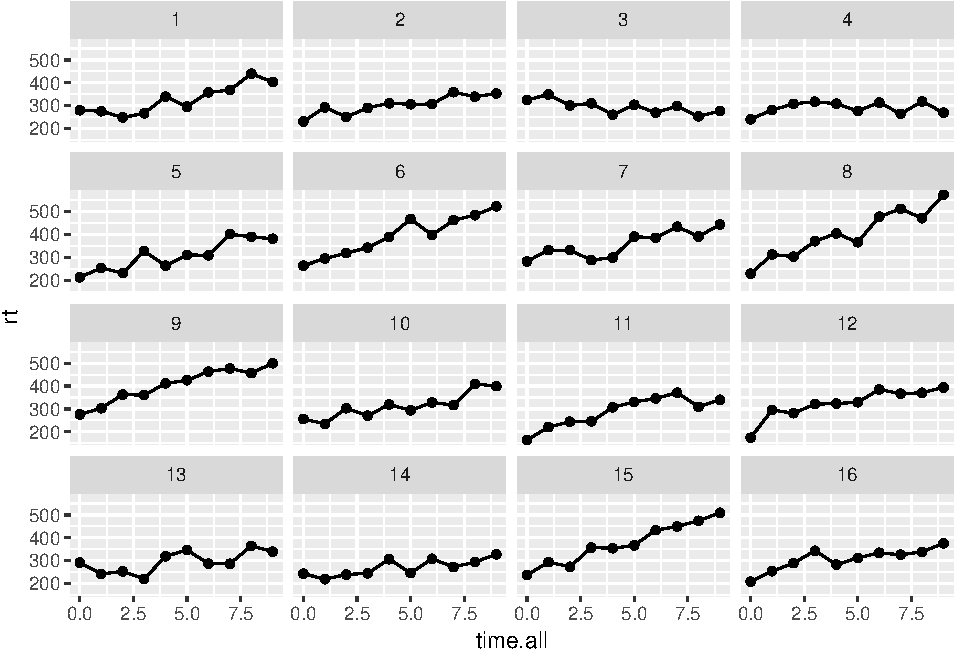
\includegraphics{MixedModelsTutorials_files/figure-latex/unnamed-chunk-3-1.pdf}

\section{Run model and compare to simulation
settings}\label{run-model-and-compare-to-simulation-settings}

Below is the appropriate model, which includes a random slope an
intercept as well as a correlation between the two. To compare with the
simulation values, first focus on the ``Random Effects'' section. This
is where to find the between-subject variances for the slope and
intercept as well as an estimate of the correlation between the two. The
within-subject variance is also in this part of the output. Be generous
when comparing these estimates with the truth since only 16 subjects
with 10 observations each went into the analysis and the estimates are
likely noisy. Recall from the \(G\) matrix above that the between
subject variance for the intercept was set to \(24^2\), the between
subject variance for the slope was \(10^2\) and the correlation between
the two was 0. The variances roughly match the estimates, specifically
26.19\(^2\) and 9.77\(^2\). The correlation is estimated at -0.33. Later
the topic of testing and simplifying random effects structures will be
covered. Last, the within-subject variance was set to 30 in the
simulations and is the Residual entry (last row) in the Random Effects
section, 28.42\(^2\).

Moving on to the fixed effects column, our simulated intercept and slope
values were 251 and 10, respectively. The estimates are pretty close:
253.56 and 16.59. Also take note of the degrees of freedom column. Why
only 15? This actually makes a lot of sense when thinking about the two
stage model. In the first stage a separate slope and intercept are
estimated for each subject and then the second stage averages these.
With 16 estimates, the degrees of freedom for an average would be 15, so
this makes sense. Always report and ask others to report degrees of
freedom, because it is a quick way to sense whether their random effects
structure may have not been correct. More on this below.

\begin{Shaded}
\begin{Highlighting}[]
\KeywordTok{summary}\NormalTok{(}\KeywordTok{lmer}\NormalTok{(rt~time.all +}\StringTok{ }\NormalTok{(}\DecValTok{1}\NormalTok{+time.all |subid.all), dat))}
\end{Highlighting}
\end{Shaded}

\begin{verbatim}
## Linear mixed model fit by REML. t-tests use Satterthwaite's method [
## lmerModLmerTest]
## Formula: rt ~ time.all + (1 + time.all | subid.all)
##    Data: dat
## 
## REML criterion at convergence: 1588.5
## 
## Scaled residuals: 
##      Min       1Q   Median       3Q      Max 
## -2.43358 -0.64266  0.03094  0.72321  2.18928 
## 
## Random effects:
##  Groups    Name        Variance Std.Dev. Corr 
##  subid.all (Intercept) 685.73   26.186        
##            time.all     95.49    9.772   -0.33
##  Residual              807.84   28.423        
## Number of obs: 160, groups:  subid.all, 16
## 
## Fixed effects:
##             Estimate Std. Error      df t value Pr(>|t|)    
## (Intercept)  253.559      7.765  15.000  32.653 2.38e-15 ***
## time.all      16.594      2.565  15.000   6.469 1.06e-05 ***
## ---
## Signif. codes:  0 '***' 0.001 '**' 0.01 '*' 0.05 '.' 0.1 ' ' 1
## 
## Correlation of Fixed Effects:
##          (Intr)
## time.all -0.405
\end{verbatim}

\section{Omitting random effects can inflate Type I
error}\label{omitting-random-effects-can-inflate-type-i-error}

Omitting the random slope often a very bad idea. Generally, all
within-subject variables that are continuous should be included as
random effects unless there are convergence issues because there aren't
enough data to estimate them. Definitely check out this paper by
\href{https://www.sciencedirect.com/science/article/pii/S0749596X17300013}{Matusheck
and others} as well as my
\href{https://www.youtube.com/watch?v=pDNEgcl0YhI}{video} to learn about
simplifying the random effects structure. Below the random slope is
omitted and the biggest impact is on the degrees of freedom, which are
quite large now! Of course this results in a much smaller p-value.
Generally there is a risk of inflated type I errors when omitting a
random effect. It is best to start with a fully specified random effects
structure and simplify if need be. This is why it is a good idea to
report degrees of freedom and make sure they are reported when reviewing
manuscripts.

\begin{Shaded}
\begin{Highlighting}[]
\NormalTok{bad.model =}\StringTok{ }\KeywordTok{lmer}\NormalTok{(rt~time.all +}\StringTok{ }\NormalTok{(}\DecValTok{1} \NormalTok{|subid.all), dat)}
\KeywordTok{summary}\NormalTok{(bad.model)  }
\end{Highlighting}
\end{Shaded}

\begin{verbatim}
## Linear mixed model fit by REML. t-tests use Satterthwaite's method [
## lmerModLmerTest]
## Formula: rt ~ time.all + (1 | subid.all)
##    Data: dat
## 
## REML criterion at convergence: 1666.7
## 
## Scaled residuals: 
##      Min       1Q   Median       3Q      Max 
## -2.53803 -0.64128 -0.00096  0.67704  2.71143 
## 
## Random effects:
##  Groups    Name        Variance Std.Dev.
##  subid.all (Intercept) 1771     42.08   
##  Residual              1634     40.42   
## Number of obs: 160, groups:  subid.all, 16
## 
## Fixed effects:
##             Estimate Std. Error      df t value Pr(>|t|)    
## (Intercept)  253.559     12.082  21.768   20.99 6.23e-16 ***
## time.all      16.594      1.113 143.000   14.91  < 2e-16 ***
## ---
## Signif. codes:  0 '***' 0.001 '**' 0.01 '*' 0.05 '.' 0.1 ' ' 1
## 
## Correlation of Fixed Effects:
##          (Intr)
## time.all -0.414
\end{verbatim}

\section{Summary}\label{summary}

The goal of this document was to shed some light on the two stage random
effects structure to aid in understanding the output of lmer. In
addition, the importance of including random effects was shown. Omitting
random effects can greatly inflate the Type I error. If you have
question about this document, please post to the MumfordBrainStats
Facebook page.

\chapter{Video 4: The Two-stage temptation: Why don''t we just use the
summary statistics
approach??}\label{video-4-the-two-stage-temptation-why-dont-we-just-use-the-summary-statistics-approach}

\section{Introduction}\label{introduction-2}

Although the two-stage formulation is a great way to conceptualize the
mixed model, it also might inspire a shortcut for data analysis: the
two-stage summary statistics approach. For those familiar with fMRI
data, this is exactly what is done to analyze those data due to the
complexity and structure of the data. The approaches vary greatly across
software packages where the SPM approach is most similar to what will be
done here, but I will not be making comparisons with or between fMRI
software. There is a
\href{https://www.ncbi.nlm.nih.gov/pubmed/19463958}{related paper},
written by myself and others that compares the models of different fMRI
software packages.

There are many reasons why the all-in-one mixed model, which I will just
call a mixed model or MM from now on, is better than using the two-stage
summary statistics approach (called 2SSS from now on). For one, you
cannot incorporate within- and between-subject parameters as easily in a
2SSS. Also, you are not allowed simplified or more complex random
effects structures. For example, there may be cases where a
within-subject variable will not be specified as random and you cannot
really do this using 2SSS. Also crossed and nested random effects, which
will be covered later if you are not already familiar with them, do not
always fit into the 2SSS framework. The most compelling reason for the
user might be that a mixed model takes about one line of code versus
many lines of code for the summary statistics approach.

\paragraph{Regularization: key
difference}\label{regularization-key-difference}

What about when the 2SSS and MM formulations are quite close? How does
the mixed model result differ? Sometimes they'll be almost identical,
but other times they will be quite different. Why? The short answer is
the within-subject values related to the fixed effects are regularized
in a mixed model and that is the focus here. This is a bit of a
confusing statement because within-subject estimates are not actually
estimated! Assume we are working with the sleepstudy data, which would
include a within- and between-subject variability. Recall the mixed
model equation, \[Y_i = X_i\beta + Z_ib_i + \epsilon_i,\] where \(Y_i\)
is the dependent variable for subject \(i\), \(X_i\) is the design
matrix for the fixed effects (see earlier document for more detail),
\(\beta\) is the \emph{group} parameter vector, \(Z_i\) is a matrix for
the random effects, \(b_i\) are the random effects describing
between-subject variability, and \(\epsilon_i\) is describes the
within-subject variability. There are not any within-subject parameters
estimated in this model. The term, \(b_i\) is a random variable that
describes the between-subject distribution, \(b_i \sim N(0, G)\).
Importantly, the \(b_i\) are not estimated, but the corresponding
covariance of the \(b_i\), \(G\), is estimated and serves as the
between-subject variability estimate. See previous lessons for more
details. Although the subject specific estimates are not estimated, the
subjects with less data will contribute less to the estimate of the
group parameter, \(\beta\). Much, much more exploration will be done on
this topic as time goes on.

For now I would like to illustrate what the regularization looks like
for means, but there isn't a perfect way to illustrate it. Typically the
regularization is shown by comparing within-subject estimates to
predicted within-subject estimates from the mixed model, based on values
called BLUPS or best linear unbiased predictors. Some are not fans of
this term, so I will simply refer to these as conditional modes,
following the notation used by Douglas Bates, the author of the lme4
library. As stated in a draft of his book, ``it is an appealing acronym,
I don't find the term particularly instructive (what is a `linear
unbiased predictor' and in what context are these the `best'?) and
prefer the term conditional mode.'' (book can be found
\href{http://webcom.upmf-grenoble.fr/LIP/Perso/DMuller/M2R/R_et_Mixed/documents/Bates-book.pdf}{here}
at the time of this writing). The reason why this isn't the perfect way
of illustrating regularization is because it doesn't perfectly reflect
how the regularization ends up impacting the group-level results. That
will be the focus in the future, but now the goal is to understand that
there is regularization happening.

The specific goal of the simulations below is to understand the impact
of regularization by looking at estimates based on within-subject
averages from the first stage of 2SSS and the conditional modes from
mixed models. The first level estimates from 2SSS will be referred to as
OLS (Ordinary Least Squares) estimates or \(\hat\beta_i^{OLS}\) and the
conditional modes will be called just that or referred to as
\(\hat\beta_i\).

\paragraph{What is a conditional
mode?}\label{what-is-a-conditional-mode}

In an effort to keep equations at a minimum, I will explain conditional
model conceptually. For more information I recommend looking at the
Bates book I linked to above or the textbook,
\href{https://www.amazon.com/Applied-Longitudinal-Analysis-Garrett-Fitzmaurice/dp/0470380276}{``Applied
Longitudinal Analysis'' by Fitzmaurice, Laird and Ware}. To understand
the difficulty of this problem, remind yourself that typically when we
have a random variable that follows a distribution, say
\(X \sim N(\mu, \sigma^2)\), we focus on the estimation of \(\mu\) and
\(\sigma^2\). Asking what value \(X\) is doesn't even make much sense,
since it is a a random variable. What can be done is to use the mode of
the distribution as a prediction of \(X\), which is where the ``mode''
in ``conditional mode'' comes from. The conditioning part is somewhat
simple. The mixed model equation above describes the distribution of
\(Y_i\) but we want the distribution of \(b_i\) for a specific subject,
\(i\). To get at this, the distribution of the random effects
conditional on the \emph{data}, \(Y\), is used. The part of this process
that is very different from when we estimate things, is that
\emph{estimated} parameters (within-subject variance, between-subject
covariance and fixed effects) are substituted in place of the truth in
the distributions in order to derive these modes instead of the true
values because they are unknown. This introduces an additional source of
variability. The take-away is simply, again, the within-subject
estimates are not estimated by default in a mixed model but we can
predict them using conditional modes. These predictions can be quite
noisy because they rely on estimates of parameters in order to specify
the conditional distribution.

Next, some fake data will be generated and used to estimate some
conditional modes and start building intuition about the regularization
in mixed models. Fake data are used for the convenience of knowing the
truth.

\subsection{Simulated data}\label{simulated-data}

The simulated data consist of 10 subjects where 5 have 50 observations
and 5 only have 5 observations from some type of behavioral experiment
measuring reaction time. As in the last lesson, the two-stage random
effects formulation will be used to simulate the data.

\begin{Shaded}
\begin{Highlighting}[]
\KeywordTok{library}\NormalTok{(lme4)}
\KeywordTok{library}\NormalTok{(lmerTest)}
\KeywordTok{library}\NormalTok{(ggplot2)}
\CommentTok{# Simulate true subject-specific means:}
\NormalTok{nsub =}\StringTok{ }\DecValTok{10}
\NormalTok{btwn.sub.sd =}\StringTok{ }\DecValTok{10}
\CommentTok{#within-subject means }
\NormalTok{win.means =}\StringTok{ }\KeywordTok{rnorm}\NormalTok{(nsub, }\DataTypeTok{mean =} \DecValTok{250}\NormalTok{, }\DataTypeTok{sd =} \NormalTok{btwn.sub.sd)}

\CommentTok{# Simualte data for each subject by wiggling around their means}
\NormalTok{win.sub.sd =}\StringTok{ }\DecValTok{20}
\CommentTok{# The following indicates how many data per subject, the first 5 only have 5 observations.}
\NormalTok{n.per.sub =}\StringTok{ }\KeywordTok{rep}\NormalTok{(}\DecValTok{50}\NormalTok{, nsub)}
\NormalTok{n.per.sub[}\DecValTok{1}\NormalTok{:}\DecValTok{5}\NormalTok{] =}\StringTok{ }\DecValTok{5}
\NormalTok{rt =}\StringTok{ }\KeywordTok{c}\NormalTok{()}
\NormalTok{subid =}\StringTok{ }\KeywordTok{c}\NormalTok{()}
\NormalTok{for (i in }\DecValTok{1}\NormalTok{:nsub)\{}
  \NormalTok{rt.loop =}\StringTok{ }\KeywordTok{rnorm}\NormalTok{(n.per.sub[i], win.means[i], }\DataTypeTok{sd =} \NormalTok{win.sub.sd)}
  \NormalTok{rt =}\StringTok{ }\KeywordTok{c}\NormalTok{(rt, rt.loop)}
  \NormalTok{subid =}\StringTok{ }\KeywordTok{c}\NormalTok{(subid, }\KeywordTok{rep}\NormalTok{(i, n.per.sub[i]))}
\NormalTok{\}}
\NormalTok{dat =}\StringTok{ }\KeywordTok{data.frame}\NormalTok{(subid, rt)}
\end{Highlighting}
\end{Shaded}

Here is a plot of the resulting data. As you can see the first five
subjects have much less data than the rest of the subjects. This was
done on purpose to illustrate the regularization since the factor that
impacts the regularization is the amount of data within-subject. There
is much more to this, but it will be covered in the following lessons.

\begin{Shaded}
\begin{Highlighting}[]
\KeywordTok{ggplot}\NormalTok{(dat, }\KeywordTok{aes}\NormalTok{(}\DataTypeTok{x=}\KeywordTok{as.factor}\NormalTok{(subid), }\DataTypeTok{y =} \NormalTok{rt)) +}\StringTok{ }\KeywordTok{geom_boxplot}\NormalTok{() +}\StringTok{ }\KeywordTok{geom_jitter}\NormalTok{(}\DataTypeTok{shape=}\DecValTok{16}\NormalTok{, }\DataTypeTok{position=}\KeywordTok{position_jitter}\NormalTok{(}\FloatTok{0.2}\NormalTok{)) +}\StringTok{ }\KeywordTok{xlab}\NormalTok{(}\StringTok{"Subject"}\NormalTok{)+}\KeywordTok{ylab}\NormalTok{(}\StringTok{"RT"}\NormalTok{)}
\end{Highlighting}
\end{Shaded}

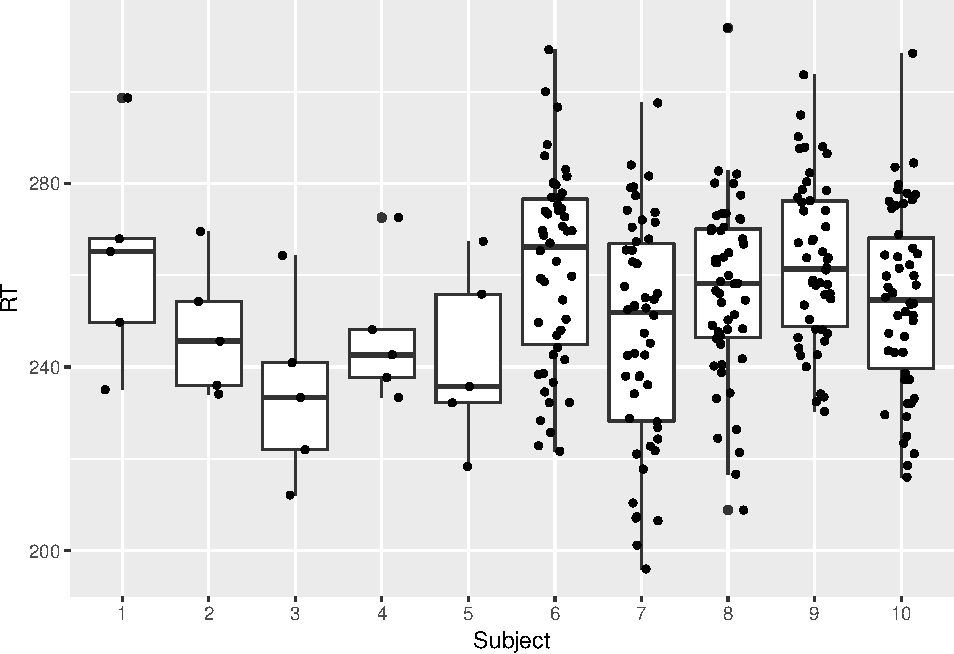
\includegraphics{MixedModelsTutorials_files/figure-latex/unnamed-chunk-9-1.pdf}

\subsection{2-stage summary statistics approach compared to predicted
subject effects from
lmer}\label{stage-summary-statistics-approach-compared-to-predicted-subject-effects-from-lmer}

Now that the data have been generated, the 2SSS uses a within-subject
OLS linear regression model to obtain the within-subject means,
\(\hat\beta_i{OLS}\) and then these are averaged in a second OLS model
to obtain the group estimates. The following runs these two stages and
also estimates the proper mixed model.

\begin{Shaded}
\begin{Highlighting}[]
\CommentTok{# Stage 1}
\NormalTok{stage1.est =}\StringTok{ }\KeywordTok{rep}\NormalTok{(}\OtherTok{NA}\NormalTok{, nsub)}
\NormalTok{for (i in }\DecValTok{1}\NormalTok{:nsub)\{}
  \CommentTok{# Estimating the mean RT via OLS}
  \NormalTok{mod.loop =}\StringTok{ }\KeywordTok{lm}\NormalTok{(rt ~}\StringTok{ }\DecValTok{1}\NormalTok{, dat[dat$subid==i,])}
  \NormalTok{stage1.est[i] =}\StringTok{ }\NormalTok{mod.loop$coef[}\DecValTok{1}\NormalTok{]}
\NormalTok{\}}

\CommentTok{#Stage 2}
\KeywordTok{summary}\NormalTok{(}\KeywordTok{lm}\NormalTok{(stage1.est ~}\StringTok{ }\DecValTok{1}\NormalTok{))}
\end{Highlighting}
\end{Shaded}

\begin{verbatim}
## 
## Call:
## lm(formula = stage1.est ~ 1)
## 
## Residuals:
##      Min       1Q   Median       3Q      Max 
## -17.1940  -4.7550  -0.5041   8.5768  11.5654 
## 
## Coefficients:
##             Estimate Std. Error t value Pr(>|t|)    
## (Intercept)  251.754      3.047   82.62 2.82e-14 ***
## ---
## Signif. codes:  0 '***' 0.001 '**' 0.01 '*' 0.05 '.' 0.1 ' ' 1
## 
## Residual standard error: 9.636 on 9 degrees of freedom
\end{verbatim}

\begin{Shaded}
\begin{Highlighting}[]
\NormalTok{## Proper mixed model}
\NormalTok{mod.lmer =}\StringTok{ }\KeywordTok{lmer}\NormalTok{(rt ~}\StringTok{ }\DecValTok{1} \NormalTok{+}\StringTok{ }\NormalTok{(}\DecValTok{1}\NormalTok{|subid), dat)}
\KeywordTok{summary}\NormalTok{(mod.lmer)}
\end{Highlighting}
\end{Shaded}

\begin{verbatim}
## Linear mixed model fit by REML. t-tests use Satterthwaite's method [
## lmerModLmerTest]
## Formula: rt ~ 1 + (1 | subid)
##    Data: dat
## 
## REML criterion at convergence: 2449.6
## 
## Scaled residuals: 
##      Min       1Q   Median       3Q      Max 
## -2.54753 -0.69671  0.02651  0.72996  2.80661 
## 
## Random effects:
##  Groups   Name        Variance Std.Dev.
##  subid    (Intercept)  39.81    6.309  
##  Residual             423.42   20.577  
## Number of obs: 275, groups:  subid, 10
## 
## Fixed effects:
##             Estimate Std. Error      df t value Pr(>|t|)    
## (Intercept)  253.885      2.638   6.206   96.25 4.35e-11 ***
## ---
## Signif. codes:  0 '***' 0.001 '**' 0.01 '*' 0.05 '.' 0.1 ' ' 1
\end{verbatim}

Comparing the lm summary to the fixed effects summary from the lmer
model, the results are almost identical. Although this makes it tempting
for many to use 2SSS instead of a mixed model, the next series of videos
will set these two modeling approaches apart.

For practice, find the within- and between-subject variance estimates in
the lmer summary and compare to the true values used in the simulation.

\subsection{OLS versus conditional
modes}\label{ols-versus-conditional-modes}

To see the impact of regularization it is necessary to predict the
subject-specific values from lmer. As mentioned above, these values are
not estimated in any way shape or form during the modeling process
above. In the following, the code asks lmer for these predicted values.

\begin{Shaded}
\begin{Highlighting}[]
\CommentTok{# Mixed model conditional modes}
\NormalTok{mmcm =}\StringTok{ }\KeywordTok{coef}\NormalTok{(mod.lmer)$subid[, }\DecValTok{1}\NormalTok{]}
\end{Highlighting}
\end{Shaded}

The following plot compares the mixed model estimates based on the
conditional mean (MMCM, orange) in orange to the within-subject OLS
estimates (OLS, blue) from the first stage of the 2SSS. The true mean
was\ldots{}.well, the reader should practice understanding the above
code by finding that themselves. Once you've located that value above,
you will notice that the orange dots (MMCM) are shrunken toward the
overall group mean compared to the blut OLS estimates. That is a result
of the regularization. Recall the first 5 subjects had much less data
than the last 5 subjects, which means there's more likely to be
\emph{more} regularization for the first 5 subjects. I will introduce an
equation that describes this exactly in the next lesson, but for now
just note the basic trend. It is easiest to see if comparing subject 1
to subject 9. In both cases their within-subject OLS estimates are
almost identical, but teh MMCM estimate for subject 1 is much smaller!
This is reflecting the fact that subject 1 had much less data than
subject 9.

\begin{Shaded}
\begin{Highlighting}[]
\NormalTok{subject =}\StringTok{ }\KeywordTok{rep}\NormalTok{(}\KeywordTok{c}\NormalTok{(}\DecValTok{1}\NormalTok{:nsub), }\DecValTok{2}\NormalTok{)}
\NormalTok{estimate =}\StringTok{ }\KeywordTok{c}\NormalTok{(mmcm, stage1.est)}
\NormalTok{estimate.type =}\StringTok{ }\KeywordTok{rep}\NormalTok{(}\KeywordTok{c}\NormalTok{(}\StringTok{"MMCM"}\NormalTok{, }\StringTok{"OLS"}\NormalTok{), }\DataTypeTok{each =} \NormalTok{nsub)}
\NormalTok{dat.sub.est =}\StringTok{ }\KeywordTok{data.frame}\NormalTok{(subject, estimate, estimate.type)}

\CommentTok{# Nice colorblind-friendly pallette}
\CommentTok{# http://www.cookbook-r.com/Graphs/Colors_(ggplot2)/#a-colorblind-friendly-palette}
\NormalTok{cbPalette <-}\StringTok{ }\KeywordTok{c}\NormalTok{(}\StringTok{"#E69F00"}\NormalTok{, }\StringTok{"#56B4E9"}\NormalTok{, }\StringTok{"#009E73"}\NormalTok{, }\StringTok{"#F0E442"}\NormalTok{, }\StringTok{"#0072B2"}\NormalTok{, }\StringTok{"#D55E00"}\NormalTok{, }\StringTok{"#CC79A7"}\NormalTok{,}\StringTok{"#999999"}\NormalTok{)}


\KeywordTok{ggplot}\NormalTok{(dat.sub.est, }\KeywordTok{aes}\NormalTok{(}\DataTypeTok{x =} \NormalTok{subject, }\DataTypeTok{y =} \NormalTok{estimate, }
                        \DataTypeTok{color =} \NormalTok{estimate.type)) +}
\StringTok{  }\KeywordTok{geom_point}\NormalTok{()+}\StringTok{ }\KeywordTok{scale_colour_manual}\NormalTok{(}\DataTypeTok{values=}\NormalTok{cbPalette) +}\StringTok{ }\KeywordTok{xlab}\NormalTok{(}\StringTok{"Subject"}\NormalTok{)+}\KeywordTok{ylab}\NormalTok{(}\StringTok{"RT"}\NormalTok{) +}\StringTok{ }\KeywordTok{labs}\NormalTok{(}\DataTypeTok{color =} \StringTok{"Estimate Type"}\NormalTok{) +}\StringTok{ }
\StringTok{  }\KeywordTok{scale_x_continuous}\NormalTok{(}\DataTypeTok{breaks =} \KeywordTok{seq}\NormalTok{(}\DecValTok{0} \NormalTok{, }\DecValTok{10}\NormalTok{, }\DecValTok{1}\NormalTok{), }\DataTypeTok{minor_breaks=}\KeywordTok{seq}\NormalTok{(}\DecValTok{0}\NormalTok{, }\DecValTok{10}\NormalTok{,}\DecValTok{1}\NormalTok{))}
\end{Highlighting}
\end{Shaded}

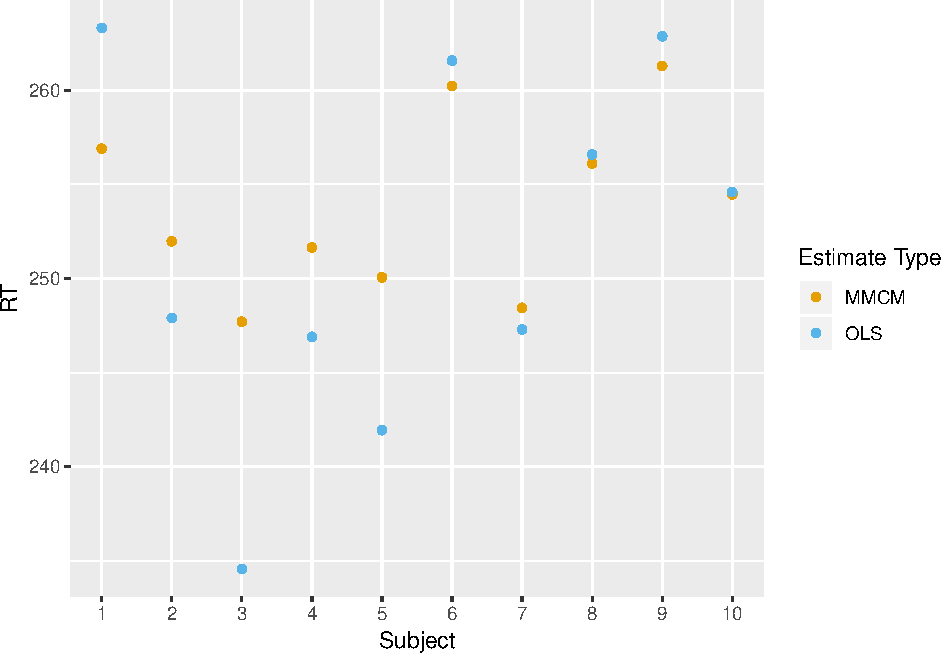
\includegraphics{MixedModelsTutorials_files/figure-latex/unnamed-chunk-12-1.pdf}

\subsection{Summary and what's next}\label{summary-and-whats-next}

This document is just a taste of what is to come. This is just a
beginning to convince folks analyzing data that data analysis can be
done better without using the two-stage summary statistics model, so
don't be tempted! Sure, this is how data are analyzed in the fMRI world,
but that's a special exception.

Although not a perfect way to view the phenomenon, conditional
mode-based within-subject estimates from mixed models help in
understanding the regularization that happens in the mixed model
framework. On the surface it can be thought of as trying to stabilize
the estimate from subjects with less data. The important take away for
now is that this is driven by the amount of data within-subject.

What inspired this series is that when I explained this point to my
colleague she immediately wanted to know how this regularization might
impact her between-subject analyses. For example, what if in the fake
data above the first 5 subjects were patients and the last 5 were
controls. It is a reasonable scenario that some patients may have less
data than controls, which is definitely the case for my colleague's
data. If the patients' estimates are shrunken toward the overall mean
because they have less data, could that introduce false positives or
reduce power? A really great question! That is what the focus will be in
the next series of lessons where I will use simulated data to compared
different modeling approaches. It will also reveal the misleading nature
of these conditional mode estimates.

\end{document}
